\section{设计要求}
设计普通型弹簧压力表,其技术要求为:
\subsection{测量范围}
测量下限制为0,测量上限制为:6。单位为MPa(${\approx}10kgf/cm^2$)
\subsection{精度等级}
精度等级:1.5级
\subsection{外形尺寸}
外形尺寸如\autoref{figure1.1}所示:
\begin{figure}[!htbp]
    \centering
    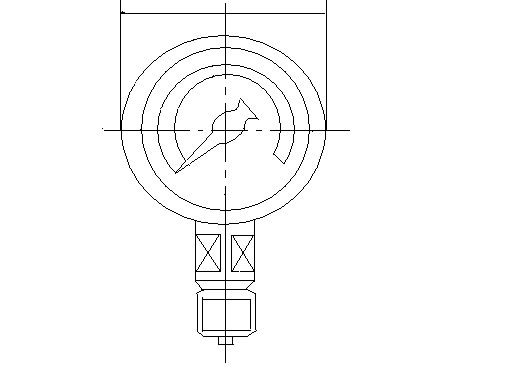
\includegraphics[width =0.45\textwidth]{figures/1.1.1.png}
    \caption{}
\end{figure}
\begin{figure}[!htbp]
    \centering
    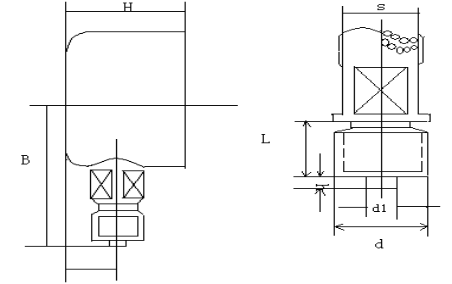
\includegraphics[width =0.65\textwidth]{figures/1.1.2.png}
    \caption{表壳外形尺寸}
    \label{figure1.1}
\end{figure}
\newline
接头位置为径向;表壳无边;表壳公称直径D=100mm;$H{\le}60mm$,
\begin{equation}
{B{\le}100mm,a=M20{\times}1.5,S=17_{-0.28}^{\circ},\\L=20_{{\pm}0.52},h=5_{{\pm}0.30},d_{1}=6_{-0.30}}\nonumber
\end{equation}
\subsection{标尺特性}
等分分度;标度角:$270^{\circ}$;
\begin{table}[!htbp]
    \centering
\caption{测量上限值与最小分度值的关系}
\label{tab:1.1}
    \begin{tabular}{|>{\centering\arraybackslash}p{0.2\linewidth}|>{\centering\arraybackslash}p{0.1\linewidth}|>{\centering\arraybackslash}p{0.1\linewidth}|>{\centering\arraybackslash}p{0.1\linewidth}|>{\centering\arraybackslash}p{0.1\linewidth}|>{\centering\arraybackslash}p{0.1\linewidth}|>{\centering\arraybackslash}p{0.1\linewidth}|} \hline 
         测量上限值&0.06&0.1&0.16&0.25&0.4&0.6\\ \hline 
         测量下限值&0.001&0.002&0.005&0.005&0.01&0.01\\ \hline 
         测量上限值&1&1.6&2.5&4&0.6& \\ \hline 
         测量下限值&0.02&0.05&0.05&0.1&0.1& \\ \hline
    \end{tabular}
\end{table}
\newline

由\autoref{tab:1.1},由于我们设计的压力表量程上限为0.4Mpa,所以选择最小分度值为0.01.所以,所设计的压力表最小分度值为0.01MPa(${\approx}10kgf/cm^2$)
